%DGraph_counter_example_original

\begin{figure*}[t]
  \centering
  \begin{subfigure}[c]{0.5\textwidth}
 %   \centering
    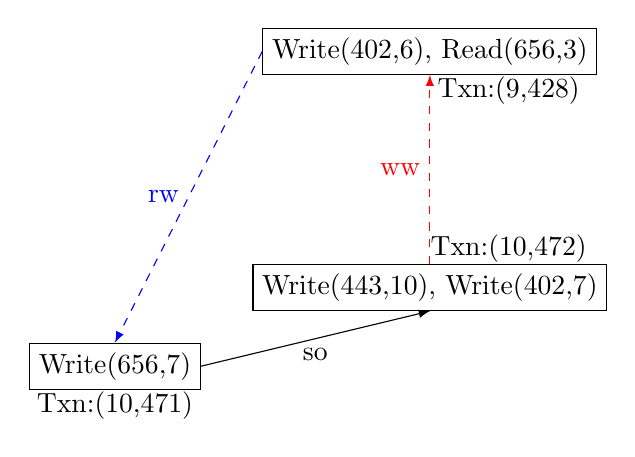
\begin{tikzpicture}[model/.style = {draw, minimum size = 15pt},  node distance = 0.5cm and 1.5cm]
        \node[model] (10472) at (0,0) {Write(443,10), Write(402,7)};
        \node (textof10472) at (1,0.5) {Txn:(10,472)};
        \node[model] (9428) at (0,3) {Write(402,6), Read(656,3)};
        \node (textof9428) at (1,2.5) {Txn:(9,428)};
        \node[model] (10471) at (-4,-1) {Write(656,7)};
        \node (textof10471) at (-4,-1.5) {Txn:(10,471)};
        \path[dashed, -latex, color=red] (10472.north) edge node[left] {ww} (9428.south); 
        \path[dashed, -latex, color=blue] (9428.west) edge node[left] {rw} (10471.north); 
        \path[-latex] (10471.east) edge node[below] {so} (10472.south); 
    \end{tikzpicture}
    \caption{The original output of the violation in DGraph.}
    \label{fig:original-DGraph}
  \end{subfigure}
\end{figure*}